%!TEX root=document.tex


\section{{\large \SeeDB\ } Design}
\label{sec:system_architecture}

In this section, we present the \SeeDB\ architecture, starting with an
overview followed by a detailed discussion of its frontend component.
The backend component, which does the heavy lifting for \SeeDB\ is described
in detail in the next section.

\subsection{{\large \SeeDB} architecture overview}
\label{subsec:overview}

In this work, we explored two distinct implementations of \SeeDB: one as a
layer on top of a relational database system (row store as well as column
store) and another as a stand alone in-memory system. 
While the former
implementation restricts optimization opportunities by virtue of being outside
the database, our design permits \SeeDB\ to be used in conjunction with a
variety of existing database systems.
The in-memory implementation, on the other hand, allows us to finely control
which views are evaluated in parallel and perform incremental pruning of views
as the execution proceeds. 
In this section, we present the high-level architecture of
\SeeDB\ without focusing on the specific execution engine (DBMS-based or main
memory). In the subsequent sections, we discuss both execution engines in
detail.

\begin{figure}[htb]
\vspace{-10pt}
\centerline{
\hbox{\resizebox{9cm}{!}{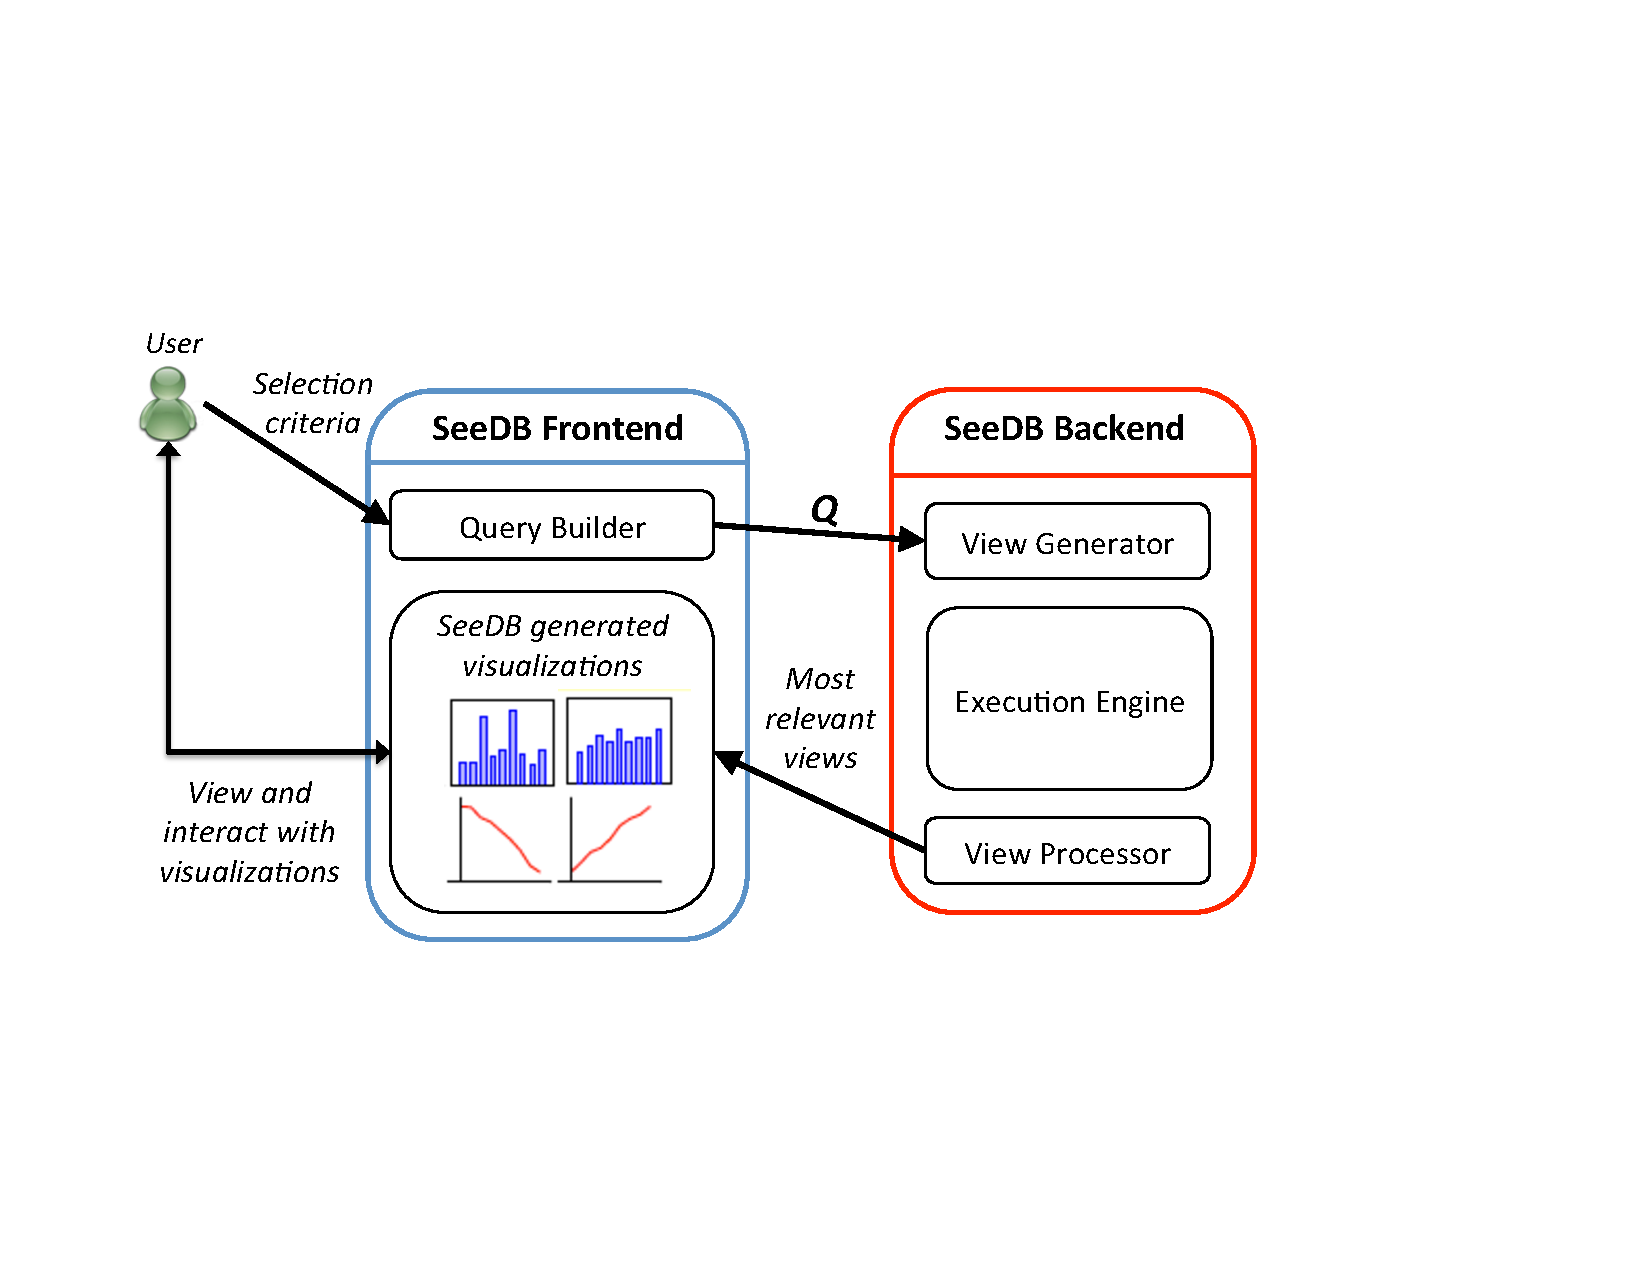
\includegraphics[trim=10mm 20mm 10mm 40mm,
clip=true]{Images/seedb-architecture.pdf}}}}
\caption{SeeDB Architecture}
\label{fig:sys-arch}
\vspace{-12pt}
\end{figure} 

\SeeDB\ is comprised of two main parts: a frontend and a backend. 
The frontend is a ``thin client''
that is used to issue queries, display visualizations  and allow basic interactions
with the visualizations. 
The backend, in contrast, performs all the computation required to generate and select views
to be recommended. 
Figure \ref{fig:sys-arch}
depicts the architecture of our system.

Once the analyst issues a query via the frontend, the backend takes over.
First, the View Generator queries the metadata information in the system for
information such as table sizes, column types and correlations between column
values. 
It then uses this metadata and the incoming query to prune the space
of possible views and generate stubs of the remaining views (discussed further
in Section \ref{}). 
The view stubs are then sent to the execution engine that evaluates the views to
identify the top views of interest.

In the DBMS-based execution engine (Section \ref{}), the view stubs are passed
through the optimizer that identifies the best ways to combine the queries to minimize
execution time.
Once the views have been optimized, the views are rewritten as SQL queries and
executed against the underlying database. 
The results of these queries are
processed to update the view stubs and compute view utility. 
Once all the queries have been processed, the top-k views are returned to the
frontend.

In the main-memory execution engine, \SeeDB\ makes a single pass through the
data (either read from disk or already present in memory) and keeps running
estimates of utility for each of the views stubs obtained from the View
Generator. 
As the engine processes more of the data, the utility estimates become more
accurate and \SeeDB\ uses various pruning heuristics to prune out views on the fly.
By the time the full data has been processed, \SeeDB\ has identified the top-k
views with the largest utility that are then returned to the frontend.

Ones the \SeeDB\ backend has identified the best visualizations, the \SeeDB\
frontend generates and displays visualizations for each of these views. We now
discuss each \SeeDB\ module in detail.
